\section{Computational Results}\label{sec:computational_results}

The aim of computational results presented in this section is to verify that the proposed approach is valid for complex instances coming from real-life applications, that describe an extended network with many trains, and an extended time horizon with a dense discretisation. We also want to validate that our algorithm achieves good results in real-time settings, where running times are limited to few seconds.

To this end, we have initially considered 23 instances, generated from three different real-world railway networks, provided to us by Alstom Transport. The first set of instances (N01-N13) describes a relatively small network chatacterised by the presence of single track lines used in both directions. The second set of six instances (L01-L06) refers to a busy regional network with a large main station and several smaller stations. Finally, the third set includes four instances (P01-P04) describing a high-speed network with frequent long-distance trains.

\Cref{tbl:instances_description} outlines the main characteristics of the instances considered. Column ``\# Trains'' lists the number of trains present in the instance; ``\# Nodes'' is the number of resources, i.e., the cardinality of the set $\Nodes$ in the network graph $\NetGraph$ (before time expansion); ``Time horizon'' is the span, in hours, of the planning horizon; ``Discretisation'' is the time discretisation step used, expressed in seconds; ``\# Conflicts'' is the sum of the number of conflicts (as described in \Cref{ssec:conflicts}: illegal overtaking, hard capacity violation, headway time violation) plus the number of violated mandatory time dependencies, given as input in the current train plan.

\begin{table}
    \begin{center}
        \begin{tabular}{lrrrrr}
            \textbf{Name} & \textbf{\# Trains} & \textbf{\# Nodes} & \textbf{Time horizon (h)} & \textbf{Discretisation (s)} & \textbf{\# Conflicts} \\
            \hline
            N01 & 28 & 108 & 2 & 15 & 24 \\
            N02 & 16 & 167 & 2 & 15 & 15 \\
            N03 & 28 & 172 & 2 & 15 & 36 \\
            N04 & 17 & 112 & 2 & 15 & 4 \\
            N05 & 18 & 112 & 2 & 15 & 12 \\
            N06 & 17 & 112 & 2 & 15 & 2 \\
            N07 & 28 & 126 & 2 & 15 & 12 \\
            N08 & 30 & 132 & 2 & 15 & 5 \\
            N09 & 28 & 130 & 2 & 15 & 4 \\
            N10 & 30 & 135 & 2 & 15 & 3 \\
            N11 & 15 & 137 & 1 & 15 & 1 \\
            N12 & 20 & 153 & 1 & 15 & 2 \\
            N13 & 33 & 135 & 4 & 15 & 37 \\
            L01 & 139 & 664 & 1 & 15 & 20 \\
            L02 & 103 & 631 & 0.75 & 15 & 54 \\
            L03 & 131 & 666 & 1 & 15 & 62 \\
            L04 & 132 & 675 & 1 & 15 & 25 \\
            L05 & 151 & 673 & 1.25 & 15 & 97 \\
            L06 & 133 & 671 & 1 & 15 & 38 \\
            P01 & 55 & 859 & 1 & 10 & 22 \\
            P02 & 55 & 814 & 1 & 10 & 22 \\
            P03 & 61 & 742 & 1 & 10 & 72 \\
            P04 & 71 & 731 & 1 & 10 & 70 \\
            \hline
        \end{tabular}
    \end{center}
    \caption{Main characteristics of the instances provided by Alstom.}\label{tbl:instances_description}
\end{table}

In \Cref{ssec:ptuning} we perform parameter tuning, to determine which graph sparsification methods and initial sortings are more likely to produce good solutions when used together with each policy (RVNS or Tabu) and time limit (2s or 10s). In \Cref{ssec:ptest} we run a simple parallel version of the algorithm on the 23 instances, using the tuned parameters.

In order to validate and benchmark our approach, we also generated new instances, which we are making publicly available. We used the network topology of the 2012 RAS Competition instances (see \citet{informs2012problem}), in two configurations: in the first (letter ``N''), each segment is modelled as a separate resource, giving an N-track scenario; in the second (letter ``S'') parallel tracks are not modelled separately, but as a single resource with the appropriate capacity, giving a single-track scenario. We generated 15 instances of each type, divided in groups of 3. The nominal timetable is the same for each group, while the disturbances change, so to have 5 different forecast timetables for each nominal one. Because the RAS network is smaller than the networks used in the instances of \Cref{tbl:instances_description}, in order to obtain feasible nominal timetables we had to either use fewer trains (instances of the first group), or a longer time horizon with a more coarse discretisation (instances of the second and third groups). These instances are available at \cite{alberto_santini_2017_322571}.

%\Cref{fig:ras_inst_micro} shows the network topology of the RAS instances in the more microscopic representation, while \Cref{fig:ras_inst_macro} shows the same network in the more macrospoic representations.
%\begin{sidewaysfigure}
  \begin{center}
    \resizebox{\textwidth}{!}{%
    \begin{tikzpicture}
      \node (n0) at (0,0) {\huge\textbullet};
      \node (n1) at (0.3,0) {\huge\textbullet};
      \node (n3) at (2.3,0) {\huge\textbullet};
      \node (n5) at (2.6,0) {\huge\textbullet};
      \node (n6) at (7.6,0) {\huge\textbullet};
      \node (n7) at (11.6,0) {\huge\textbullet};
      \node (n8) at (11.9,0) {\huge\textbullet};
      \node (n10) at (13.9,0) {\huge\textbullet};
      \node (n12) at (14.2,0) {\huge\textbullet};
      \node (n13) at (19.2,0) {\huge\textbullet};
      \node (n14) at (24.2,0) {\huge\textbullet};
      \node (n15) at (24.5,0) {\huge\textbullet};
      \node (n17) at (26.5,0) {\huge\textbullet};
      \node (n19) at (26.8,0) {\huge\textbullet};
      \node (n20) at (31.8,0) {\huge\textbullet};
      \node (n21) at (37.8,0) {\huge\textbullet};
      \node (n22) at (38.1,0) {\huge\textbullet};
      \node (n25) at (40.1,0) {\huge\textbullet};
      \node (n26) at (40.4,0) {\huge\textbullet};
      \node (n27) at (41.4,0) {\huge\textbullet};
      \node (n28) at (41.7,0) {\huge\textbullet};
      \node (n30) at (44.7,0) {\huge\textbullet};
      \node (n31) at (47.7,0) {\huge\textbullet};
      \node (n32) at (48,0) {\huge\textbullet};
      \node (n34) at (50,0) {\huge\textbullet};
      \node (n36) at (50.3,0) {\huge\textbullet};
      \node (n37) at (53.5,0) {\huge\textbullet};
      \node (n40) at (53.8,0) {\huge\textbullet};
      \node (n43) at (55.8,0) {\huge\textbullet};
      \node (n45) at (58.8,0) {\huge\textbullet};
      \node (n47) at (59.1,0) {\huge\textbullet};
      \node (n49) at (63.1,0) {\huge\textbullet};
      \node (n50) at (63.4,0) {\huge\textbullet};
      \node (n52) at (65.4,0) {\huge\textbullet};
      \node (n55) at (65.7,0) {\huge\textbullet};
      \node (n56) at (67.7,0) {\huge\textbullet};
      \node (n58) at (68,0) {\huge\textbullet};
      \node (n60) at (71,0) {\huge\textbullet};
      \node (n62) at (74,0) {\huge\textbullet};
      \node (n64) at (74.3,0) {\huge\textbullet};
      \node (n66) at (77.3,0) {\huge\textbullet};
      \node (n68) at (80.3,0) {\huge\textbullet};
      \node (n69) at (80.6,2) {\huge\textbullet};
      \node (n70) at (85.6,2) {\huge\textbullet};
      \node (n71) at (90.6,2) {\huge\textbullet};
      \node (n72) at (90.9,2) {\huge\textbullet};
      \node (n74) at (93.9,2) {\huge\textbullet};
      \node (n76) at (94.2,2) {\huge\textbullet};
      \node (n77) at (98.2,2) {\huge\textbullet};
      \node (n78) at (102.2,2) {\huge\textbullet};
      \node (n79) at (102.5,2) {\huge\textbullet};
      \node (n81) at (104.5,2) {\huge\textbullet};
      \node (n38) at (104.8,2) {\huge\textbullet};
      \node (n39) at (109.8,2) {\huge\textbullet};

      \node (n41) at (53.8,2) {\huge\textbullet};
      \node (n42) at (55.8,2) {\huge\textbullet};
      \node (n44) at (58.8,2) {\huge\textbullet};
      \node (n46) at (59.1,2) {\huge\textbullet};
      \node (n48) at (63.1,2) {\huge\textbullet};
      \node (n54) at (67.7,2) {\huge\textbullet};
      \node (n57) at (68,2) {\huge\textbullet};
      \node (n59) at (71,2) {\huge\textbullet};
      \node (n61) at (74,2) {\huge\textbullet};
      \node (n63) at (74.3,2) {\huge\textbullet};
      \node (n65) at (77.3,2) {\huge\textbullet};
      \node (n67) at (80.3,2) {\huge\textbullet};

      \node (n2) at (0.3,2) {\huge\textbullet};
      \node (n4) at (2.3,2) {\huge\textbullet};
      \node (n16) at (24.5,2) {\huge\textbullet};
      \node (n18) at (26.5,2) {\huge\textbullet};
      \node (n33) at (48,2) {\huge\textbullet};
      \node (n35) at (50,2) {\huge\textbullet};
      \node (n51) at (63.4,-2) {\huge\textbullet};
      \node (n53) at (65.4,-2) {\huge\textbullet};
      \node (n80) at (102.5,0) {\huge\textbullet};
      \node (n82) at (104.5,0) {\huge\textbullet};

      \draw[-] (n0.center) -- (n1.center) -- (n3.center) -- (n5.center) -- (n6.center) -- (n7.center) -- (n8.center) -- (n10.center) -- (n12.center) -- (n13.center) -- (n14.center) -- (n15.center) -- (n17.center) -- (n19.center);
      \draw[-] (n19.center) -- (n20.center) -- (n21.center) -- (n22.center) -- (n25.center) -- (n26.center) -- (n27.center) -- (n28.center) -- (n30.center) -- (n31.center) -- (n32.center) -- (n34.center) -- (n36.center);
      \draw[-] (n36.center) -- (n37.center) -- (n40.center) -- (n43.center) -- (n45.center) -- (n47.center) -- (n49.center) -- (n50.center) -- (n52.center) -- (n55.center) -- (n56.center) -- (n58.center) -- (n60.center);
      \draw[-] (n60.center) -- (n62.center) -- (n64.center) -- (n66.center) -- (n68.center) -- (n69.center) -- (n70.center) -- (n71.center) -- (n72.center) -- (n74.center) -- (n76.center) -- (n77.center) -- (n78.center);
      \draw[-] (n78.center) -- (n79.center) -- (n81.center) -- (n38.center) -- (n39.center);
      \draw[-] (n37.center) -- (n41.center) -- (n42.center) -- (n44.center) -- (n46.center) -- (n48.center) -- (n54.center) -- (n57.center) -- (n59.center) -- (n61.center) -- (n63.center) -- (n65.center) -- (n67.center) -- (n69.center);
      \draw[-] (n0.center) -- (n2.center) -- (n4.center) -- (n5.center);
      \draw[-] (n14.center) -- (n16.center) -- (n18.center) -- (n19.center);
      \draw[-] (n31.center) -- (n33.center) -- (n35.center) -- (n36.center);
      \draw[-] (n49.center) -- (n51.center) -- (n53.center) -- (n55.center);
      \draw[-] (n78.center) -- (n80.center) -- (n82.center) -- (n38.center);
      \draw[-] (n45.center) -- (n46.center);
      \draw[-] (n44.center) -- (n47.center);
      \draw[-] (n54.center) -- (n58.center);
      \draw[-] (n56.center) -- (n57.center);
    \end{tikzpicture}}
    \caption{Network topology of the RAS-based instances. In this representation, each track is modelled separately.}\label{fig:ras_inst_micro}
    \vspace{1em}
    \resizebox{\textwidth}{!}{%
    \begin{tikzpicture}
      \node (n0) at (0,0) {\huge\textbullet};
      \node (n1) at (0.3,0) {\huge\textbullet};
      \node (n3) at (2.3,0) {\huge\textbullet};
      \node (n5) at (2.6,0) {\huge\textbullet};
      \node (n6) at (7.6,0) {\huge\textbullet};
      \node (n7) at (11.6,0) {\huge\textbullet};
      \node (n8) at (11.9,0) {\huge\textbullet};
      \node (n10) at (13.9,0) {\huge\textbullet};
      \node (n12) at (14.2,0) {\huge\textbullet};
      \node (n13) at (19.2,0) {\huge\textbullet};
      \node (n14) at (24.2,0) {\huge\textbullet};
      \node (n15) at (24.5,0) {\huge\textbullet};
      \node (n17) at (26.5,0) {\huge\textbullet};
      \node (n19) at (26.8,0) {\huge\textbullet};
      \node (n20) at (31.8,0) {\huge\textbullet};
      \node (n21) at (37.8,0) {\huge\textbullet};
      \node (n22) at (38.1,0) {\huge\textbullet};
      \node (n25) at (40.1,0) {\huge\textbullet};
      \node (n26) at (40.4,0) {\huge\textbullet};
      \node (n27) at (41.4,0) {\huge\textbullet};
      \node (n28) at (41.7,0) {\huge\textbullet};
      \node (n30) at (44.7,0) {\huge\textbullet};
      \node (n31) at (47.7,0) {\huge\textbullet};
      \node (n32) at (48,0) {\huge\textbullet};
      \node (n34) at (50,0) {\huge\textbullet};
      \node (n36) at (50.3,0) {\huge\textbullet};
      \node (n37) at (53.5,0) {\huge\textbullet};
      \node (n40) at (53.8,0) {\huge\textbullet};
      \node (n43) at (55.8,0) {\huge\textbullet};
      \node (n45) at (58.8,0) {\huge\textbullet};
      \node (n47) at (59.1,0) {\huge\textbullet};
      \node (n49) at (63.1,0) {\huge\textbullet};
      \node (n50) at (63.4,0) {\huge\textbullet};
      \node (n52) at (65.4,0) {\huge\textbullet};
      \node (n55) at (65.7,0) {\huge\textbullet};
      \node (n56) at (67.7,0) {\huge\textbullet};
      \node (n58) at (68,0) {\huge\textbullet};
      \node (n60) at (71,0) {\huge\textbullet};
      \node (n62) at (74,0) {\huge\textbullet};
      \node (n64) at (74.3,0) {\huge\textbullet};
      \node (n66) at (77.3,0) {\huge\textbullet};
      \node (n68) at (80.3,0) {\huge\textbullet};
      \node (n69) at (80.6,0) {\huge\textbullet};
      \node (n70) at (85.6,0) {\huge\textbullet};
      \node (n71) at (90.6,0) {\huge\textbullet};
      \node (n72) at (90.9,0) {\huge\textbullet};
      \node (n74) at (93.9,0) {\huge\textbullet};
      \node (n76) at (94.2,0) {\huge\textbullet};
      \node (n77) at (98.2,0) {\huge\textbullet};
      \node (n78) at (102.2,0) {\huge\textbullet};
      \node (n79) at (102.5,0) {\huge\textbullet};
      \node (n81) at (104.5,0) {\huge\textbullet};
      \node (n38) at (104.8,0) {\huge\textbullet};
      \node (n39) at (109.8,0) {\huge\textbullet};
      \draw[-] (n0.center) -- (n1.center) -- (n3.center) -- (n5.center) -- (n6.center) -- (n7.center) -- (n8.center) -- (n10.center) -- (n12.center) -- (n13.center) -- (n14.center) -- (n15.center) -- (n17.center) -- (n19.center);
      \draw[-] (n19.center) -- (n20.center) -- (n21.center) -- (n22.center) -- (n25.center) -- (n26.center) -- (n27.center) -- (n28.center) -- (n30.center) -- (n31.center) -- (n32.center) -- (n34.center) -- (n36.center);
      \draw[-] (n36.center) -- (n37.center) -- (n40.center) -- (n43.center) -- (n45.center) -- (n47.center) -- (n49.center) -- (n50.center) -- (n52.center) -- (n55.center) -- (n56.center) -- (n58.center) -- (n60.center);
      \draw[-] (n60.center) -- (n62.center) -- (n64.center) -- (n66.center) -- (n68.center) -- (n69.center) -- (n70.center) -- (n71.center) -- (n72.center) -- (n74.center) -- (n76.center) -- (n77.center) -- (n78.center);
      \draw[-] (n78.center) -- (n79.center) -- (n81.center) -- (n38.center) -- (n39.center);
    \end{tikzpicture}}
  \end{center}
  \caption{Network topology of the RAS-based instances. In this representation, each set of parallel tracks is modelled as one single resource.}\label{fig:ras_inst_macro}
\end{sidewaysfigure}


To ease the comparison with other algorithms that might be developped in the future, we did not consider problem-specific features such as time dependencies, and splits and merges. The conflicts that can arise, therefore, are limited to headway, hard and soft capacity, crossing, and overtake violations. Soft violations are penalised with a simple linear function. \Cref{tbl:ras_instances_description} describes the features of the generated instances; columns ``H'', ``O'', and ``C'' give a detailed breakdown of the type of conflicts: headways, overtake, and hard capacity, respectively. In \Cref{ssec:ptest} we apply the tuned parallel algorithm to the new instances, similarly to what we do for the proprietary instances.

\begin{table}
  \begin{center}
    \begin{tabular}{lrrrrrr}
      & & & & \multicolumn{3}{c}{\textbf{\# Conflicts}} \\
      \textbf{Name} & \textbf{\# Trains} & \textbf{Time horizon (h)} & \textbf{Discretisation (s)} & \textbf{H} & \textbf{O} & \textbf{C} \\
      \hline
      N-1-1 & 7  & 4  & 15 & 0 & 0 & 6 \\
      N-1-2 & 7  & 4  & 15 & 63 & 0 & 43 \\
      N-1-3 & 7  & 4  & 15 & 35 & 2 & 41 \\
      N-1-4 & 7  & 4  & 15 & 35 & 1 & 42 \\
      N-1-5 & 7  & 4  & 15 & 0 & 0 & 32 \\
      N-2-1 & 12 & 12 & 60 & 2 & 0 & 3 \\
      N-2-2 & 12 & 12 & 60 & 4 & 0 & 6 \\
      N-2-3 & 12 & 12 & 60 & 2 & 0 & 4 \\
      N-2-4 & 12 & 12 & 60 & 0 & 0 & 7 \\
      N-2-5 & 12 & 12 & 60 & 6 & 0 & 13 \\
      N-3-1 & 24 & 12 & 60 & 4 & 0 & 25 \\
      N-3-2 & 24 & 12 & 60 & 105 & 0 & 53 \\
      N-3-3 & 24 & 12 & 60 & 0 & 0 & 6 \\
      N-3-4 & 24 & 12 & 60 & 103 & 0 & 89 \\
      N-3-5 & 24 & 12 & 60 & 0 & 0 & 10 \\
      S-1-1 & 7  & 4  & 15 & 0 & 0 & 3 \\
      S-1-2 & 7  & 4  & 15 & 32 & 0 & 22 \\
      S-1-3 & 7  & 4  & 15 & 4 & 1 & 28 \\
      S-1-4 & 7  & 4  & 15 & 30 & 1 & 24 \\
      S-1-5 & 7  & 4  & 15 & 2 & 0 & 19 \\
      S-2-1 & 12 & 12 & 60 & 0 & 0 & 2 \\
      S-2-2 & 12 & 12 & 60 & 2 & 0 & 2 \\
      S-2-3 & 12 & 12 & 60 & 6 & 0 & 5 \\
      S-2-4 & 12 & 12 & 60 & 0 & 0 & 4 \\
      S-2-5 & 12 & 12 & 60 & 2 & 0 & 4 \\
      S-3-1 & 24 & 12 & 60 & 0 & 0 & 21 \\
      S-3-2 & 24 & 12 & 60 & 59 & 0 & 25 \\
      S-3-3 & 24 & 12 & 60 & 0 & 0 & 4 \\
      S-3-4 & 24 & 12 & 60 & 60 & 0 & 60 \\
      S-3-5 & 24 & 12 & 60 & 2 & 0 & 12 \\
      \hline
    \end{tabular}
    \caption{Main characteristics of the instances generated starting from the 2012 RAS Competition instances.}\label{tbl:ras_instances_description}
  \end{center}
\end{table}

The tests presented in this section have been run on a dual-core 3.2GHz Intel i5 machine, with 7803MB of RAM. The CPU configuration and the L1, L2 and L3 cache sizes are detailed in \Cref{fig:cputopo}, as produced by the software Hwloc (\citet{Broquedis2010}).

\begin{figure}
  \begin{center}
    \includegraphics[width=0.33\textwidth]{figures/cputopo.png}
  \end{center}
  \caption{Schematic hardware configuration of the test machine.}\label{fig:cputopo}
\end{figure}

\subsection{Parameter tuning}\label{ssec:ptuning}

The objective of parameter tuning is to measure the impact of the sparsification methods and the sorting criteria introduced in \Cref{sec:solution_algorithm}, on real-time applications of the algorithm.

We ran six sets of experiments overall, in order to determine which combinations of sparsification and sorting are particularly effective with the RVNS and Tabu policies. For each of these two policies, the three sets of experiments only vary in the hard time limit given to the algorithm. The first two time limits are of 2 and 10 seconds (real-time); the third time limit is of 60 seconds, and is used to provide better solutions that can be used as a baseline for comparisons.

For each set of experiments, the tests were run on all the 23 Alstom instances. For each instance, we tried all combinations of sparsification methods and initial sortings, using the parameters described in \Cref{sec:solution_algorithm}. In total, we had 19 possible settings for the sparsification methods and 7 possible sortings, giving 133 tests for each policy, time limit and instance, giving a grand total of $133 \cdot 2 \cdot 3 \cdot 23 = 18\;\!354$ runs.

\begin{sidewaystable}\footnotesize
    \begin{center}
        \begin{tabular}{lrrrrrrrrrrrr}
            & \multicolumn{3}{c}{\textbf{Tabu 2s}} & \multicolumn{3}{c}{\textbf{Tabu 10s}} & \multicolumn{3}{c}{\textbf{RVNS 2s}} & \multicolumn{3}{c}{\textbf{RVNS 10s}} \\
            \cmidrule(lr){2-4}\cmidrule{5-7}\cmidrule(lr){8-10}\cmidrule(lr){11-13}
            \textbf{Sparsification} &
            \textbf{CF} & \textbf{Dev} & \textbf{CF Dev} &
            \textbf{CF} & \textbf{Dev} & \textbf{CF Dev} &
            \textbf{CF} & \textbf{Dev} & \textbf{CF Dev} &
            \textbf{CF} & \textbf{Dev} & \textbf{CF Dev} \\
            \cmidrule(lr){1-1}\cmidrule(lr){2-4}\cmidrule{5-7}\cmidrule(lr){8-10}\cmidrule(lr){11-13}
            disabled       & 0.64 & 10912.64 & 1.88 & 0.78 & 593.90   & 1.33 & 0.79 & 488.43   & 10.32 & 0.80 & 370.22   & 1.43 \\
            fixed-2        & 0.70 & 16252.12 & 1.68 & 0.77 & 15374.42 & 1.35 & 0.75 & 15811.52 & 1.73  & 0.75 & 15558.96 & 1.38 \\
            fixed-3        & 0.71 & 16161.95 & 1.66 & 0.78 & 15312.86 & 1.34 & 0.75 & 15686.94 & 1.62  & 0.76 & 15528.27 & 1.42 \\
            fixed-5        & 0.74 & 15875.32 & 1.62 & 0.78 & 15321.86 & 1.32 & 0.74 & 28820.40 & 1.59  & 0.75 & 26406.56 & 1.40 \\
            linear-2       & 0.65 & 6391.54  & 1.85 & 0.80 & 339.41   & 1.36 & 0.80 & 377.08   & 10.06 & 0.80 & 370.23   & 1.45 \\
            linear-3       & 0.64 & 8725.04  & 2.06 & 0.78 & 418.67   & 1.39 & 0.79 & 599.52   & 10.20 & 0.80 & 370.24   & 1.46 \\
            linear-5       & 0.62 & 11325.47 & 1.95 & 0.77 & 739.40   & 1.43 & 0.78 & 4981.04  & 8.29  & 0.80 & 370.25   & 1.47 \\
            progressive-2  & 0.76 & 834.95   & 1.49 & 0.82 & 31.93    & 1.24 & 0.78 & 696.63   & 1.51  & 0.80 & 308.66   & 1.34 \\
            progressive-3  & 0.73 & 1348.76  & 1.41 & 0.81 & 62.66    & 1.23 & 0.80 & 493.27   & 1.55  & 0.80 & 247.19   & 1.34 \\
            progressive-5  & 0.73 & 1439.36  & 1.50 & 0.82 & 64.21    & 1.23 & 0.78 & 663.47   & 1.57  & 0.78 & 379.93   & 1.32 \\
            threshold-2-5  & 0.66 & 3977.49  & 4.29 & 0.80 & 217.94   & 1.26 & 0.80 & 406.13   & 7.95  & 0.80 & 370.16   & 1.38 \\
            threshold-2-10 & 0.67 & 3851.51  & 4.25 & 0.79 & 247.15   & 1.27 & 0.78 & 445.13   & 8.05  & 0.79 & 339.43   & 1.38 \\
            threshold-2-15 & 0.66 & 4157.31  & 4.34 & 0.79 & 310.16   & 1.27 & 0.80 & 406.14   & 7.95  & 0.80 & 370.17   & 1.38 \\
            threshold-3-5  & 0.70 & 1482.97  & 1.62 & 0.80 & 247.14   & 1.28 & 0.79 & 568.01   & 7.93  & 0.80 & 370.15   & 1.36 \\
            threshold-3-10 & 0.69 & 1627.55  & 1.63 & 0.80 & 247.15   & 1.29 & 0.78 & 475.82   & 7.99  & 0.79 & 400.89   & 1.36 \\
            threshold-3-15 & 0.68 & 1742.63  & 4.20 & 0.80 & 187.18   & 1.24 & 0.79 & 436.84   & 7.95  & 0.79 & 370.16   & 1.36 \\
            threshold-5-5  & 0.73 & 1333.08  & 1.49 & 0.81 & 93.41    & 1.22 & 0.79 & 556.38   & 3.63  & 0.79 & 308.66   & 1.34 \\
            threshold-5-10 & 0.70 & 1708.34  & 1.56 & 0.81 & 93.42    & 1.24 & 0.79 & 525.67   & 3.67  & 0.79 & 370.14   & 1.34 \\
            threshold-5-15 & 0.69 & 1750.12  & 1.58 & 0.81 & 62.70    & 1.27 & 0.79 & 525.69   & 3.69  & 0.79 & 400.89   & 1.36 \\
            \cmidrule(lr){1-1}\cmidrule(lr){2-4}\cmidrule{5-7}\cmidrule(lr){8-10}\cmidrule(lr){11-13}
        \end{tabular}
    \end{center}
    \caption{Parameter tuning results aggregated by sparsification method.}\label{tbl:par_tun_results_spars}
\end{sidewaystable}

\begin{sidewaystable}\footnotesize
    \begin{center}
        \begin{tabular}{lrrrrrrrrrrrr}
            & \multicolumn{3}{c}{\textbf{Tabu 2s}} & \multicolumn{3}{c}{\textbf{Tabu 10s}} & \multicolumn{3}{c}{\textbf{RVNS 2s}} & \multicolumn{3}{c}{\textbf{RVNS 10s}} \\
            \cmidrule(lr){2-4}\cmidrule{5-7}\cmidrule(lr){8-10}\cmidrule(lr){11-13}
            \textbf{Sorting} &
            \textbf{CF} & \textbf{Dev} & \textbf{CF Dev} &
            \textbf{CF} & \textbf{Dev} & \textbf{CF Dev} &
            \textbf{CF} & \textbf{Dev} & \textbf{CF Dev} &
            \textbf{CF} & \textbf{Dev} & \textbf{CF Dev} \\
            \cmidrule(lr){1-1}\cmidrule(lr){2-4}\cmidrule{5-7}\cmidrule(lr){8-10}\cmidrule(lr){11-13}
            Congestion         & 0.73 & 3197.61  & 1.58 & 0.80 & 2509.98 & 1.29 & 0.79 & 3535.41 & 11.38  & 0.80 & 3349.47 & 1.42 \\
            Conflict time      & 0.73 & 7938.66  & 4.92 & 0.80 & 2589.95 & 1.28 & 0.78 & 4012.83 & 9.14   & 0.78 & 3700.91 & 1.31 \\
            Length             & 0.73 & 3302.75  & 1.64 & 0.80 & 2635.49 & 1.27 & 0.78 & 3882.08 & 1.75   & 0.78 & 3791.12 & 1.44 \\
            Random             & 0.59 & 13031.87 & 2.01 & 0.81 & 2637.88 & 1.34 & 0.76 & 5482.95 & 9.27   & 0.78 & 2623.51 & 1.45 \\
            Reverse congestion & 0.74 & 5170.65  & 1.72 & 0.78 & 2589.07 & 1.29 & 0.78 & 3848.59 & 1.77   & 0.78 & 3756.94 & 1.37 \\
            Reverse speed      & 0.65 & 4110.60  & 1.61 & 0.79 & 2584.59 & 1.26 & 0.77 & 2890.27 & 1.75   & 0.77 & 2841.63 & 1.35 \\
            Speed              & 0.68 & 4105.06  & 1.70 & 0.79 & 2861.43 & 1.31 & 0.82 & 3229.39 & 4.74   & 0.82 & 3224.74 & 1.33 \\
            \cmidrule(lr){1-1}\cmidrule(lr){2-4}\cmidrule{5-7}\cmidrule(lr){8-10}\cmidrule(lr){11-13}
        \end{tabular}
    \end{center}
    \caption{Parameter tuning results aggregated by initial sorting.}\label{tbl:par_tun_results_sort}
\end{sidewaystable}

\Cref{tbl:par_tun_results_spars} and \Cref{tbl:par_tun_results_sort} show the results we obtained during parameter tuning for the two solvers, with time limits 2 and 10 seconds. In the first table the results have been aggregated by sparsification method, while in the second, they have been aggregated by sorting criterion.

Columns ``Sparsification'' (in \Cref{tbl:par_tun_results_spars}) or ``Sorting'' (in \Cref{tbl:par_tun_results_sort}) tell, respectively, for which sparsification method or sorting criterion the data is being aggregated. For each line the data are grouped in four blocks, corresponding to the four combinations of policy (Tabu or RVNS) and time limit (2s or 10s). Column ``CF'' gives the fraction of tests for which the algorithm was able to find a conflict-free schedule. Column ``Dev'' is the average deviation, calculated as $(z - z^*) / z^*$ where $z$ is the solution value obtained by the algorithm with the specified configuration, and $z^*$ is the best known solution value. This best known value comes from the 60 seconds runs that we use as baseline, and is the best value across all possible parameter combinations. Since, as explained in \Cref{sec:solution_algorithm}, the objective function has a hierarchical structure and unresolved conflicts take a very large penalty, the values in this column tend to be quite large, as one single instance for which a method was not able to produce a conflict-free schedule can increase the average considerably. This is, however, a good metric of the desirability of a method, because solving conflicts always has priority on any other measure of solution quality. In column ``CF Dev'', we similarly report the average deviation, but this time we only consider the conflict-free solutions in the average.

We want to select the best sparsification method for each policy (RVNS or Tabu) and each time limit (2s or 10s). In order to do this, it is not sufficient to take the policy with the lowest deviation, but one has to ensure that the differences in deviation are statistically relevant.

For this reason, we ran a Wilcoxon signed-rank test on each pair of sparsification methods, to measure whether their deviations across the various instances come from the same distribution or not (in this latter case, a difference in the average deviation is statistically relevant).

\begin{figure}
    \begin{subfigure}[ht]{0.5\textwidth}
        \begin{center}
            \includegraphics[width=0.95\textwidth]{figures/spars-2-tabu.png}
        \end{center}
        \caption{Policy: Tabu, time limit: 2s.}\label{sfig:wilcoxon_2_tabu}
    \end{subfigure}
    \begin{subfigure}[ht]{0.5\textwidth}
        \begin{center}
            \includegraphics[width=0.75\textwidth]{figures/spars-2-vns.png}
        \end{center}
        \caption{Policy: RVNS, time limit: 2s.}\label{sfig:wilcoxon_2_vns}
    \end{subfigure}
    \caption{Visual representation of the results of the Wilcoxon test (time limit: 2s).}\label{fig:wilcoxon_2}
\end{figure}

\begin{figure}
    \begin{subfigure}[ht]{\textwidth}
        \begin{center}
            \includegraphics[width=0.95\textwidth]{figures/spars-10-tabu.png}
        \end{center}
        \caption{Policy: Tabu, time limit: 10s.}\label{sfig:wilcoxon_10_tabu}
    \end{subfigure}
    \par\bigskip
    \begin{subfigure}[ht]{\textwidth}
        \begin{center}
            \includegraphics[width=0.75\textwidth]{figures/spars-10-vns.png}
        \end{center}
        \caption{Policy: RVNS, time limit: 10s.}\label{sfig:wilcoxon_10_vns}
    \end{subfigure}
    \caption{Visual representation of the results of the Wilcoxon test (time limit: 10s).}\label{fig:wilcoxon_10}
\end{figure}

\Cref{fig:wilcoxon_2} and \Cref{fig:wilcoxon_10} give a graphical representation of the outcomes of the Wilcoxon test. Each figure gives a representation of a directed graph. Sparsification methods are represented as nodes. An arc is drawn between two nodes if the $p$-value of the Wilcoxon test relative to two sparsifications is $<0.05$; the arc goes from the node with the better average deviation to that with the worse one. The colour and the thickness of the arc depend on the difference between the deviations: the greater the difference, the thicker and bluer the arc; on the other hand, small differences are represented by thin red-ish arcs. In particular, notice that the thickness and colour of the arc are not related with the $p$-value, which is used only as a threshold to decide whether to create the arc.

To simplify the visualisation, nodes and arcs are drawn from top to bottom, so that the best sparsifications are in the top part of the graph. Furthemore, in order to reduce the number of arcs drawn in the figure, whenever there are arcs $(M_1, M_2), (M_2, M_3)$ and $(M_1, M_3)$, this latter arc is removed. In other terms, if a method $M_1$ dominates method $M_2$, and $M_2$ dominates $M_3$, it is implicit that $M_1$ dominates $M_3$.

The sparisification methods were chosen as follows:
\begin{itemize}
    \item In the case of policy Tabu and time limit 2s (\Cref{sfig:wilcoxon_2_tabu}) the only two undominated methods are ``progressive-2'' and ``progressive-3''; since the average deviation of the former is 38.1\% smaller than that of the latter (see \Cref{tbl:par_tun_results_spars}), we decided to take ``progressive-2'' as the chosen sparsification method.
    \item For policy RVNS and time limit 2s, the only undominated method is ``linear-2'', which also has a considerably smaller deviation compared to the other methods.
    \item An interesting case is that of policy Tabu and time limit 10s (\Cref{sfig:wilcoxon_10_tabu}), as this is the case where it is most unclear which sparsification emerges as a winner. However, since the deviation of method ``progressive-2'' is the smallest, and it is 49.04\% smaller than the second-smallest one (``progressive-3''), we chose this method.
    \item Finally, for policy RVNS and time limit 10s, the three undominated methods were ``progressive-2'', ``progressive-3'', and ``threshold-5-5''. Again, since the average deviation for ``progressive-3'' is 19.92\% smaller than that for the other two (which have the same deviation), we chose that method.
\end{itemize}

\begin{table}\footnotesize%
	\tabcolsep=5pt
    \begin{center}
        \begin{tabular}{lrrrrrrrrrrrr}
            & \multicolumn{3}{c}{\textbf{Tabu 2s}} & \multicolumn{3}{c}{\textbf{Tabu 10s}} & \multicolumn{3}{c}{\textbf{RVNS 2s}}  & \multicolumn{3}{c}{\textbf{RVNS 10s}} \\
            & \multicolumn{3}{c}{\textbf{progressive-2}} & \multicolumn{3}{c}{\textbf{progressive-2}} & \multicolumn{3}{c}{\textbf{linear-2}} & \multicolumn{3}{c}{\textbf{progressive-3}} \\
            \cmidrule(lr){2-4}\cmidrule(lr){5-7}\cmidrule(lr){8-10}\cmidrule(lr){11-13}
            & \multicolumn{2}{c}{Deviation} & & \multicolumn{2}{c}{Deviation} & & \multicolumn{2}{c}{Deviation} & & \multicolumn{2}{c}{Deviation} & \\
			\cmidrule(lr){2-3}\cmidrule(lr){5-6}\cmidrule(lr){8-9}\cmidrule(lr){11-12}
			\textbf{Sorting} & Avg & Std & Best & Avg & Std & Best & Avg & Std & Best & Avg & Std & Best \\
            \cmidrule(lr){1-1}\cmidrule(lr){2-4}\cmidrule(lr){5-7}\cmidrule(lr){8-10}\cmidrule(lr){11-13}
            Congestion         & 441.45   & 2115.65 & 8 & 0.16   & 0.22    & 12 & 11.83  & 53.76   & 6 &   0.36 & 0.83    & 8 \\
            Conflict time      & 430.66   & 2063.77 & 2 & 0.22   & 0.30    &  2 & 442.05 & 2062.05 & 6 & 430.57 & 2063.81 & 5 \\
            Length             & 1076.20  & 5159.38 & 4 & 0.24   & 0.38    &  2 & 861.38 & 4127.40 & 2 & 215.53 & 1031.94 & 1 \\
            Random             & 2461.98  & 9855.31 & 3 & 0.22   & 0.31    &  2 & 227.90 & 1030.85 & 1 & 430.60 & 2063.80 & 3 \\
            Rev. Congestion    & 226.44   & 1083.85 & 3 & 0.14   & 0.16    &  2 & 646.11 & 3095.51 & 3 & 430.59 & 2063.73 & 1 \\
            Rev. Speed         & 554.88   & 1887.01 & 1 & 0.19   & 0.33    &  2 & 431.11 & 2063.69 & 3 & 215.47 & 1032.00 & 1 \\
            Speed              & 646.03   & 3095.86 & 2 & 215.37 & 1031.95 &  3 & 12.15  & 53.70   & 2 &   0.23 & 0.42    & 4 \\
            \cmidrule(lr){1-1}\cmidrule(lr){2-4}\cmidrule(lr){5-7}\cmidrule(lr){8-10}\cmidrule(lr){11-13}
        \end{tabular}
    \end{center}
    \caption{Average deviations of different sortings, for the chosen sparsification methods.}\label{tbl:chosen_spars}
\end{table}

\Cref{tbl:chosen_spars} shows the chosen sparsification methods and gives the average deviations (columns ``Avg''), together with their standard deviation (column ``Std''), obtained by employing the different initial sortings with each sparsification. Column ``Best'' tells the number of instances (out of 23) for which each sorting criterion provided the best result, compared to the other criteria in the same column.

\subsection{Parallel algorithm}\label{ssec:ptest}

\begin{table}
    \begin{center}
        \begin{tabular}{llll}
            \textbf{Tabu 2s} & \textbf{Tabu 10s} & \textbf{RVNS 2s} & \textbf{RVNS 10s} \\
            \textbf{progressive-2} & \textbf{progressive-2} & \textbf{linear-2} & \textbf{progressive-3} \\
            \hline
            \rule{0pt}{2.5ex}Congestion & Congestion & Congestion & Congestion \\
            Length & Conflict Time & Conflict Time & Conflict Time \\
            Reverse Congestion & Reverse Congestion & Reverse Congestion & Speed \\
            Random & Reverse Speed & Reverse Speed & Random \\
            \hline
        \end{tabular}
    \end{center}
    \caption{List of sorting criteria chosen for each policy and time limit, to be used in the parallel algorithm.}\label{tbl:chosen_sorts}
\end{table}

In this section we provide computational results for a very simple parallel implementation of the algorithm. We ran four sets of experiments, namely one for each combination of policy and time limit, together with the respective sparsification method chosen during parameter tuning, as described in \Cref{ssec:ptuning}. For each set, the parallel implementation simply consists of launching four parallel instances of the algorithm, each using one of four sorting criteria. When the time limit hits, the four solutions provided by the parallel instances are examined and the best one is returned as the overall solution.

The usage of parallel algorithms in operational research is well-established. We refer the reader to, e.g., \citet{clausen1999best} for parallel strategies for branch-and-bound exact algorithms, or to \citet{ropke2017palns} for a systematic analysis of the speed-ups obtained by parallelising the Adaptive Large Neighbourhood Search metaheuristic. With respect to the train rescheduling problem, \citet{iqbal2012parallel,iqbal2013multi} proposed parallel algorithms for rescheduling under disturbances.

In our case, the implementation of a parallel algorithm is motivated by the high dispersion of the solution values with respect to the average one, obtained by the different sorting methods, as witnessed by the high values of Standard Deviation reported in \Cref{tbl:chosen_spars} (this effect is more evident for the 2s time limit compared to the 10s one, and for the RVNS policy compared to the Tabu one). This means that, in practice, even the best sorting method was not able to resolve some solvable conflict, thus resulting in high solution values, due to the hierarchical nature of our objective function. Furthermore, we observed a certain complementarity in the capability of resolving conflicts across different sortings, which we see as a hint towards the parallel use of different sorting criteria.

More formally, we investigated the dependance of sorting criteria to instance characteristics via simple \emph{one-vs-all} and \emph{one-vs-one} multiclass classification algorithms provided by the library \texttt{scikit} (see, e.g., \citet{aly2005class}). These algorithms were based on the binary classifier that, for a fixed time limit, assigns an instance to an intial sorting criterion (class) if there is at least one policy (either Tabu or RVNS) for which that sorting provided the best result for that time limit. The instance features considered were the one listed in \Cref{tbl:instances_description,tbl:ras_instances_description}. Neither the \emph{one-vs-all} nor the \emph{one-vs-one} algorithm found statistically significant relationships of the sorting criteria to the instance features.

Once established the need for an algorithm that employs more than one sorting criteria at once, it is clearly important to perform a good choice of the criteria. The simplest approach would be to choose the four criteria that produce the four lowest deviations for a given policy and time limit (see \Cref{tbl:chosen_spars}). This choice, however, has not proven particularly good especially for the lowest time limit, and in one case we even had one instance (instance ``P4'' for the Tabu policy at 2s) for which not all solvable conflicts were actually resolved.

What we aim for is a choice of methods out of which, given any instance, there are high chances to find one that works reasonably well with that instance, eliminating all solvable conflicts, and therefore exploting the aforementioned complementarity. For this reason, we decided to choose the methods in a way to maximise the number of instances for which at least one of the methods chosen was the best. \Cref{tbl:chosen_sorts} lists the chosen sorting criterian for each policy and time limit.

\begin{table}\footnotesize
    \begin{center}
        \begin{tabular}{lllrrrrr}
            \textbf{Instance group} & \textbf{Algorithm} & \textbf{Sorting} & \textbf{Dev} & \textbf{Conflicts} & \textbf{Infeasible} & \textbf{Modified} & \textbf{Delay} \\
            \hline
            L   & Tabu 2s	& Random, Length, Reverse congestion    & 0.17  & 0.50 & 0.00 & 104.50 & 28.64 \\
            L   & Tabu 10s  & Reverse congestion                    & 0.11  & 0.50 & 0.00 & 104.67 & 29.00 \\
            L   & RVNS 2s	& Reverse speed                         & 0.17  & 0.50 & 0.00 & 105.67 & 33.34 \\
            L   & RVNS 10s  & Conflict time                         & 0.05  & 0.50 & 0.00 & 100.83 & 10.64 \\
            N   & Tabu 2s   & Congestion                            & 0.16  & 0.38 & 0.08 & 7.85   & 79.43 \\
            N   & Tabu 10s  & Congestion                            & 0.08  & 0.38 & 0.08 & 8.23   & 70.12 \\
            N   & RVNS 2s   & Congestion                            & 0.45  & 0.38 & 0.08 & 7.54   & 99.30 \\
            N   & RVNS 10s  & Congestion                            & 0.26  & 0.38 & 0.08 & 8.00   & 67.69 \\
            P   & Tabu 2s   & Reverse congestion                    & 0.50  & 0.00 & 0.00 & 59.25  & 247.17 \\
            P   & Tabu 10s  & Reverse speed                         & 0.03  & 0.00 & 0.00 & 59.50  & 220.52 \\
            P   & RVNS 2s   & Conflict time                         & 0.30  & 0.00 & 0.00 & 59.50  & 226.83 \\
            P   & RVNS 10s  & Congestion                            & 0.20  & 0.00 & 0.00 & 59.50  & 221.58 \\
            \hline
            \multicolumn{2}{l}{\textbf{Overall 2s}} & \textbf{Congestion} & \textbf{0.29} & \textbf{0.35} & \textbf{0.04} & \textbf{42.09} & \textbf{99.81} \\
            \multicolumn{2}{l}{\textbf{Overall 10s}} & \textbf{Congestion} & \textbf{0.14} & \textbf{0.35} & \textbf{0.04} & \textbf{41.74} & \textbf{82.56} \\
            \multicolumn{2}{l}{\textbf{Overall Tabu}} & \textbf{Congestion} & \textbf{0.15} & \textbf{0.35} & \textbf{0.04} & \textbf{42.15} & \textbf{90.45} \\
            \multicolumn{2}{l}{\textbf{Overall RVNS}} & \textbf{Congestion} & \textbf{0.27} & \textbf{0.35} & \textbf{0.04} & \textbf{41.67} & \textbf{91.92} \\
            \hline
            \multicolumn{2}{l}{\textbf{Overall}} & \textbf{Congestion} & \textbf{0.21} & \textbf{0.35} & \textbf{0.04} & \textbf{41.91} & \textbf{91.19} \\
            \hline
        \end{tabular}
        \caption{Parallel algorithm results on the Alstom instances.}\label{tbl:comp_results_alstom}
    \end{center}
\end{table}

\begin{table}\footnotesize
    \begin{center}
        \begin{tabular}{lllrrrrr}
            \textbf{Instance group} & \textbf{Algorithm} & \textbf{Sorting} & \textbf{Dev} & \textbf{Conflicts} & \textbf{Infeasible} & \textbf{Modified} & \textbf{Delay} \\
            \hline
            S-1   & Tabu 2s	  & Reverse congestion & $2.26 \cdot 10^{-2}$ & 0 & 0 & 4.60 & 132.67 \\
            S-1   & Tabu 10s  & Reverse congestion & $1.99 \cdot 10^{-2}$ & 0 & 0 & 4.60 & 131.72 \\
            S-1   & RVNS 2s	  & Reverse speed & $3.58 \cdot 10^{-2}$ & 0 & 0 & 4.60 & 134.77 \\
            S-1   & RVNS 10s  & Length, Speed & $1.64 \cdot 10^{-2}$ & 0 & 0 & 4.60 & 129.30 \\
            S-2   & Tabu 2s   & Reverse congestion & $3.97 \cdot 10^{-3}$ & 0 & 0 & 3.80 & 63.77 \\
            S-2   & Tabu 10s  & Congestion & $1.83 \cdot 10^{-3}$ & 0 & 0 & 3.80 & 60.61 \\
            S-2   & RVNS 2s   & Conflict time & $6.75 \cdot 10^{-4}$ & 0 & 0 & 3.80 & 60.04 \\
            S-2   & RVNS 10s  & Speed & $3.54 \cdot 10^{-4}$ & 0 & 0 & 3.80 & 59.80 \\
            S-3   & Tabu 2s   & Length, Congestion & $1.24 \cdot 10^{-2}$ & 0 & 0 & 5.20 & 185.33 \\
            S-3   & Tabu 10s  & Congestion & $2.65 \cdot 10^{-3}$ & 0 & 0 & 5.00 & 188.68 \\
            S-3   & RVNS 2s   & Conflict time & $7.52 \cdot 10^{-3}$ & 0 & 0 & 5.20 & 190.85 \\
            S-3   & RVNS 10s  & Congestion, Speed & $8.02 \cdot 10^{-5}$ & 0 & 0 & 5.20 & 186.63 \\
            N-1   & Tabu 2s	  & Random, Congestion & $6.91 \cdot 10^{-4}$ & 0 & 0 & 4.20 & 125.05 \\
            N-1   & Tabu 10s  & Reverse congestion & $6.91 \cdot 10^{-4}$ & 0 & 0 & 4.20 & 125.05 \\
            N-1   & RVNS 2s	  & Conflict time & $1.19 \cdot 10^{-1}$ & 0 & 0 & 3.80 & 154.79 \\
            N-1   & RVNS 10s  & Congestion & $2.25 \cdot 10^{-4}$ & 0 & 0 & 4.20 & 124.86 \\
            N-2   & Tabu 2s   & Length & $9.90 \cdot 10^{-4}$ & 0 & 0 & 4.00 & 106.31 \\
            N-2   & Tabu 10s  & Conflict time & $9.90 \cdot 10^{-4}$ & 0 & 0 & 4.00 & 106.31 \\
            N-2   & RVNS 2s   & Conflict time & $7.52 \cdot 10^{-4}$ & 0 & 0 & 4.00 & 106.42 \\
            N-2   & RVNS 10s  & Length & $1.32 \cdot 10^{-4}$ & 0 & 0 & 4.00 & 106.06 \\
            N-3   & Tabu 2s   & Reverse congestion & $2.15 \cdot 10^{-2}$ & 0 & 0 & 6.00 & 219.10 \\
            N-3   & Tabu 10s  & Conflict time & $7.14 \cdot 10^{-3}$ & 0 & 0 & 5.40 & 203.28 \\
            N-3   & RVNS 2s   & Conflict time & $9.28 \cdot 10^{-3}$ & 0 & 0 & 5.20 & 205.11 \\
            N-3   & RVNS 10s  & Speed & $7.40 \cdot 10^{-3}$ & 0 & 0 & 5.20 & 207.49 \\
            \hline
            \multicolumn{2}{l}{\textbf{Overall 2s}} & \textbf{Conflict time} &   $\mathbf{1.93 \cdot 10^{-2}}$ & \textbf{0} & \textbf{0} & \textbf{4.20} & \textbf{140.27} \\
            \multicolumn{2}{l}{\textbf{Overall 10s}} & \textbf{Congestion} &  $\mathbf{5.07 \cdot 10^{-3}}$ & \textbf{0} & \textbf{0} & \textbf{4.23} & \textbf{135.90} \\
            \multicolumn{2}{l}{\textbf{Overall Tabu}} & \textbf{Reverse congestion} & $\mathbf{7.05 \cdot 10^{-3}}$ & \textbf{0} & \textbf{0} & \textbf{4.30} & \textbf{137.32} \\
            \multicolumn{2}{l}{\textbf{Overall RVNS}} & \textbf{Conflict time} & $\mathbf{1.64 \cdot 10^{-2}}$ & \textbf{0} & \textbf{0} & \textbf{4.20} & \textbf{138.84} \\
            \hline
            \multicolumn{2}{l}{\textbf{Overall}} & \textbf{Conflict time} & $\mathbf{1.22 \cdot 10^{-2}}$ & \textbf{0} & \textbf{0} & \textbf{4.25} & \textbf{138.08} \\
            \hline
        \end{tabular}
        \caption{Parallel algorithm results on the RAS-Based instances.}\label{tbl:comp_results_ras}
    \end{center}
\end{table}

\begin{figure}
    \begin{center}
        \includegraphics[width=0.75\textwidth]{figures/mod_trains_scatter.png}
    \end{center}
    \caption{Scatter graph (without outliers) showing the correlation between solution quality and number of modified trains.}\label{fig:mod_trains_scatter}
\end{figure}

\Cref{tbl:comp_results_alstom} reports aggregate results for the parallel algorithm on the Alstom instances. Column ``Sorting'' reports which initial sorting produced the optimal solution most often, for a fixed choice of instance group and algorithm. Column ``Dev'' gives the average deviation, calculated as $(z - z^*) / z^*$ where $z$ is the solution value obtained by the algorithm, and $z^*$ is the best known solution value. Column ``Conflicts'' lists the average number of conflicts remaining in the output solution, while columns ``Infeasible'' and ``Modified'' report, respectively, the number of trains that are infeasible and whose schedule has been modified in the output solution. Finally, ``Delay'' lists the average delay (or advance, in which case the figure is $<0$) reported by trains at their final destination.

By observing the tables, it is clear that the benefit of the parallel algorithm is considerable when compared to fixed choices of sorting criteria. This is particularly evident for the 2s time limit, where the best average deviations achieved by using only one sorting (see \cref{tbl:chosen_spars}) were of 226.44 for Tabu and 11.83 for RVNS, while the parallel algorithms gives --- respectively --- 0.22 and 0.35 (see the detailed results in \Cref{tbl:tabu_res,tbl:vns_res}). In addition, by looking at the detailed results, we can notice that all four sortings selected for each set (algorithm and time limit) provide the best solution in some instances, with the ``Congestion'' sorting being the one appearing most frequently overall, and also when aggregating by policy or by time limit.

For what concerns the choice of the heuristic policy, from the detailed results we can notice that Tabu and RVNS turn out to provide the smallest instance-by-instance deviations almost the same number of times: namely, both 15 times for 2s, and 18 vs 17 times for 10s. From \Cref{tbl:comp_results_alstom} we can see, however, that Tabu provides smaller deviations, at the cost of modifying more trains. A small further reduction could be achieved by an hypothetical algorithm that ran the Tabu and RVNS policies in parallel (thereby using 8 concurrent threads): such an algorithm would achieve an average deviation of 0.17 for 2s, and 0.06 for 10s. Finally, as we clearly expected, a considerable improvement is obtained by letting the algorithm run for longer: the average deviation for all methods ran for 10s is less than half than that for all methods ran for 2s.

\Cref{fig:mod_trains_scatter} displays the relation between the deviations achieved by the parallel algorithm and the number of trains whose schedules have been modified. All the solutions described in \Cref{tbl:tabu_res} and \Cref{tbl:vns_res} are reported in the figure. The figure seems to suggest that, despite not having included the number of modified trains as a penalty term in the objective funciont (see \Cref{sssec:other_terms}) there are no solutions in which a lot of trains are modified and, despite that, bad solutions are obtained. This can be seen by noticing that the upper-right triangle of the graph is empty. In summary, the figure seem to suggest that three scenarios can happen. The first, best scenario is that a high quality solution is found and few trains are modified (bottom-left cluster of points); in the second scenario a high quality solution is found, but a lot of trains have to be modified (points on the top-left corner); finally, rarely a bad solution is found, but in this case only few trains are modified (bottom-right points).

\Cref{tbl:comp_results_ras} is analogous to \Cref{tbl:comp_results_alstom} and reports aggregate results for the parallel algorithm on the RAS-based instances. Notice that, due to the nature of the instances, the deviation are smaller compared to those reported in \Cref{tbl:comp_results_alstom}, and all conflicts were resolved in each instance. Also, the average number of modified trains is smaller for RAS instances than for Alstom instances; this is not surprising, as the number of train in the nominal timetable was also smaller. Average delays are, on the other hand, higher, probably due to the fact that the time horizon is longer for the RAS-based instances.

As in the case of the Alstom instances, there is a lot of variability in which initial sorting criterion leads to the best solution; not only some criterion works best with particular instances, but also the combination of instance and policy seems to influence the effectiveness of the sorting criterion. This confirms the negative results obtained by the classification algorithms, and the potential of a (simple) parallel implementation in order to obtain good practical results.
